\chapter{Analyse des résultats}

\section{Métrique d'évaluation IoU}
En général, Intersection over Union (IoU) (ou indice de Jaccard) est considéré comme la métrique la plus populaire pour l'évaluation de détection d'objet. Dans le domaine de la détection d'objet, IoU est utilisé pour mesurer la similarité entre la bounding box prédit $B_{p}$ et la bounding box de la vérité terrain $B_{gt}$, en mesurant l'intersection (l'aire du chevauchement) pour $B_{p}$ et $B_{gt}$, divisée par l'aire de leur union, qui est:
$$IoU=J(B_{p}, B_{gt})=\frac{aire(B_{p} \cap B_{gt})}{aire(B_{p} \cup B_{gt})}$$
 
Comme illustré en figure \ref{fig:iou_example}:

\begin{figure}[!htbp]
\center
	\subfloat{{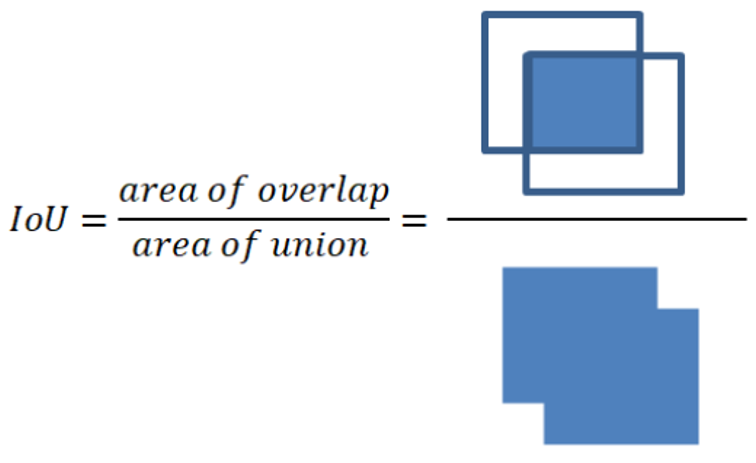
\includegraphics[scale=0.5]{IoU.png}}}
\caption{Intersection over Union (IoU)}
\label{fig:iou_example}
\end{figure}
\FloatBarrier


Dans notre cas, les bounding boxes de prédiction correspondent à la sortie de notre logiciel, ou à celle du réseau de neurones (YOLOv7). Les bounding boxes de la vérité terrain, quant à elles, correspondent à des bounding boxes annotées manuellement et qui englobe l'objet ciblé à détecter (i.e. la seiche).\\
Pour avoir la vérité terrain, nous avons utilisé LabelImg.\\
\\

Afin de classifier le résultat de la détection comme étant correcte ou non, nous comparons l'IoU à un seuil donné $T$. Donc, si $IoU > T$, alors nous pouvons considérer la détection comme étant correcte, autrement, la détection est considérée comme incorrecte.\\
Dans nos tests, nous avons fixé le seuil $T$ à 0.5.



\clearpage
\section{Analyse et comparaison}
Les valeurs IoU sont calculées pour une séquence et deux approches (filtre à particule et YOLOv7), elles sont représentées dans la table \ref{tab:results}.\\
Notre méthode avec filtre à particule a réussi à détecter la seiche dans 288 des 292 frames, équivalent à 98\% du nombre total de frames, voir figure \ref{fig:pf_results}. L'IoU varie de 0.44 à 0.87 et l'IoU moyen est de 0.74.\\
YOLOv7 a réussi à détecter la seiche dans 292 des 292 frames, équivalent à 100\% du nombre total de frames, voir figure \ref{fig:yolo_results}. L'IoU varie de 0.60 à 0.90 et l'IoU moyen est de 0.76.

\begin{table}[!htbp]
\begin{tabular}{|c|c|c|c|c|c|}
\hline
Méthode & Frames & Fréquence de détection & IoU min & IoU max & IoU mean\\
\hline
Filtre à particule & 292 & 288 (98\%) & 0.44 & 0.87 & 0.74\\
\hline
YOLOv7 & 292 & 292 (100\%) & 0.60 & 0.90 & 0.76\\
\hline
\end{tabular}
\caption{Résultats pour une même séquence en utilisant notre filtre à particule et YOLOv7.}
\label{tab:results}
\end{table}
\FloatBarrier

\begin{figure}[!htbp]
\center
	\subfloat[Frame 25]{{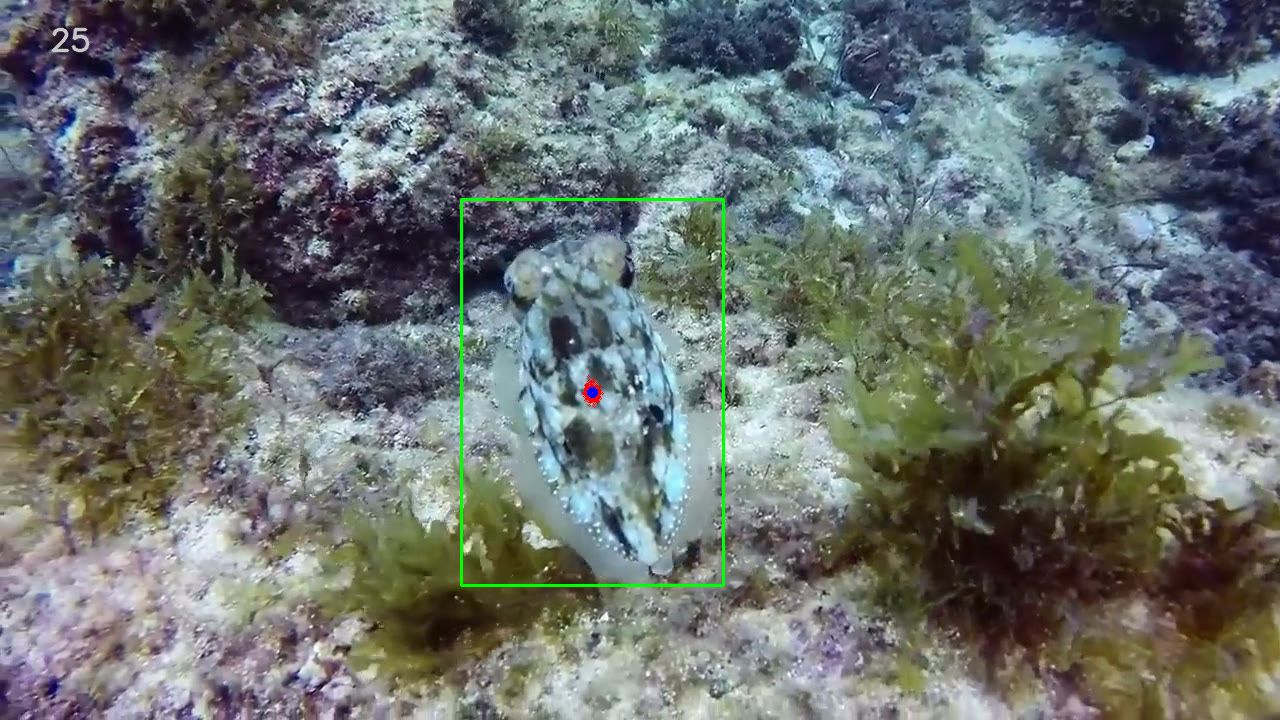
\includegraphics[scale=0.15]{result_pf_valid_1.png}}}
	\hspace{0.1cm}
	\subfloat[Frame 50]{{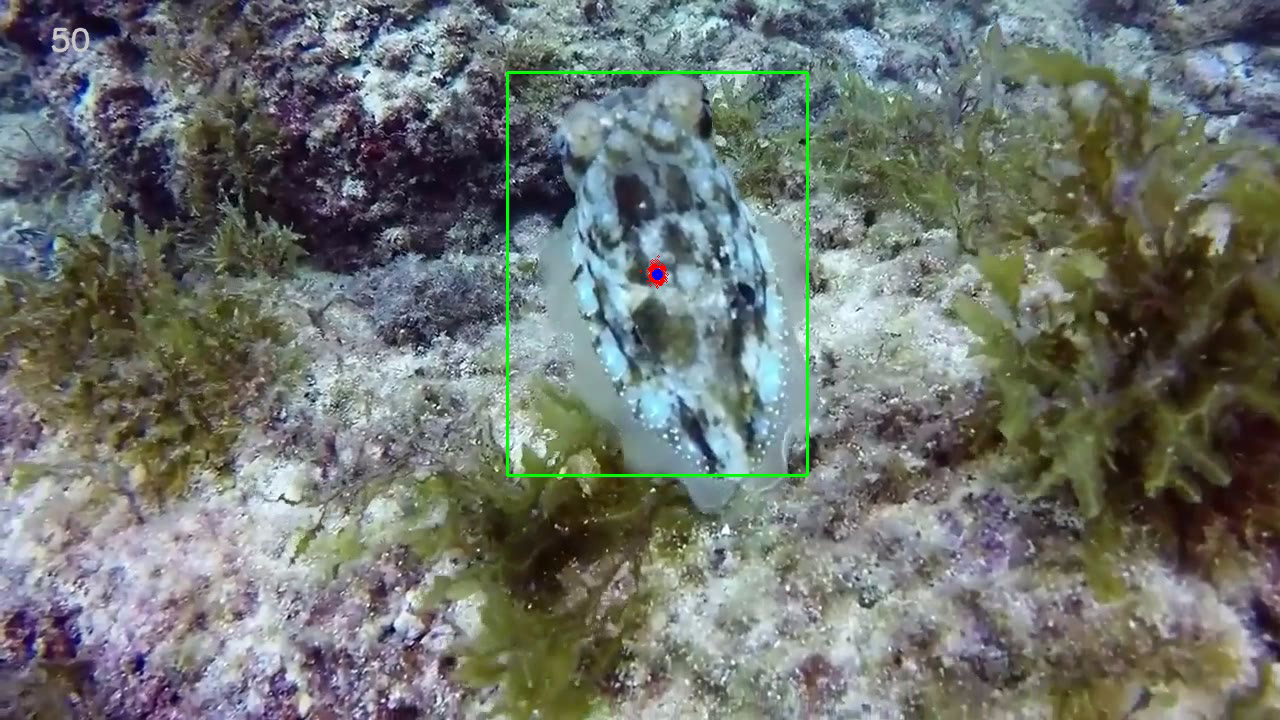
\includegraphics[scale=0.15]{result_pf_valid_2.png}}}
	\\
	\subfloat[Frame 100]{{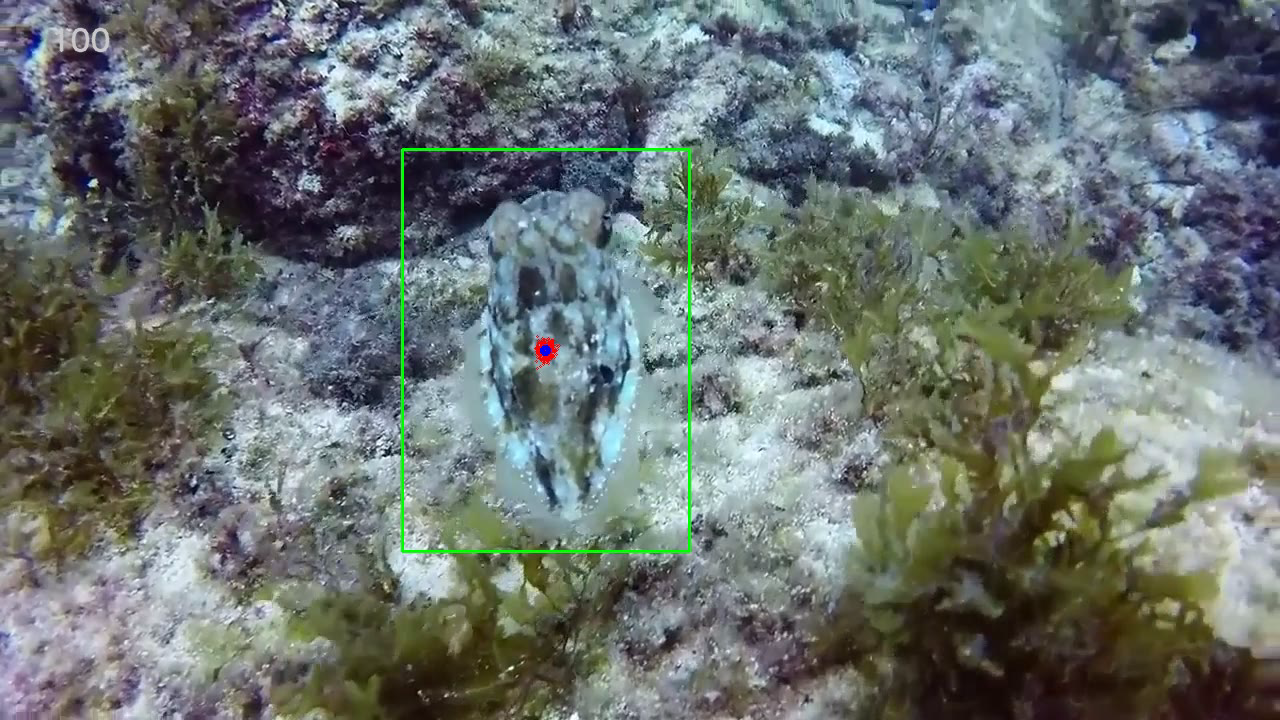
\includegraphics[scale=0.15]{result_pf_valid_3.png}}}
	\hspace{0.1cm}
	\subfloat[Frame 150]{{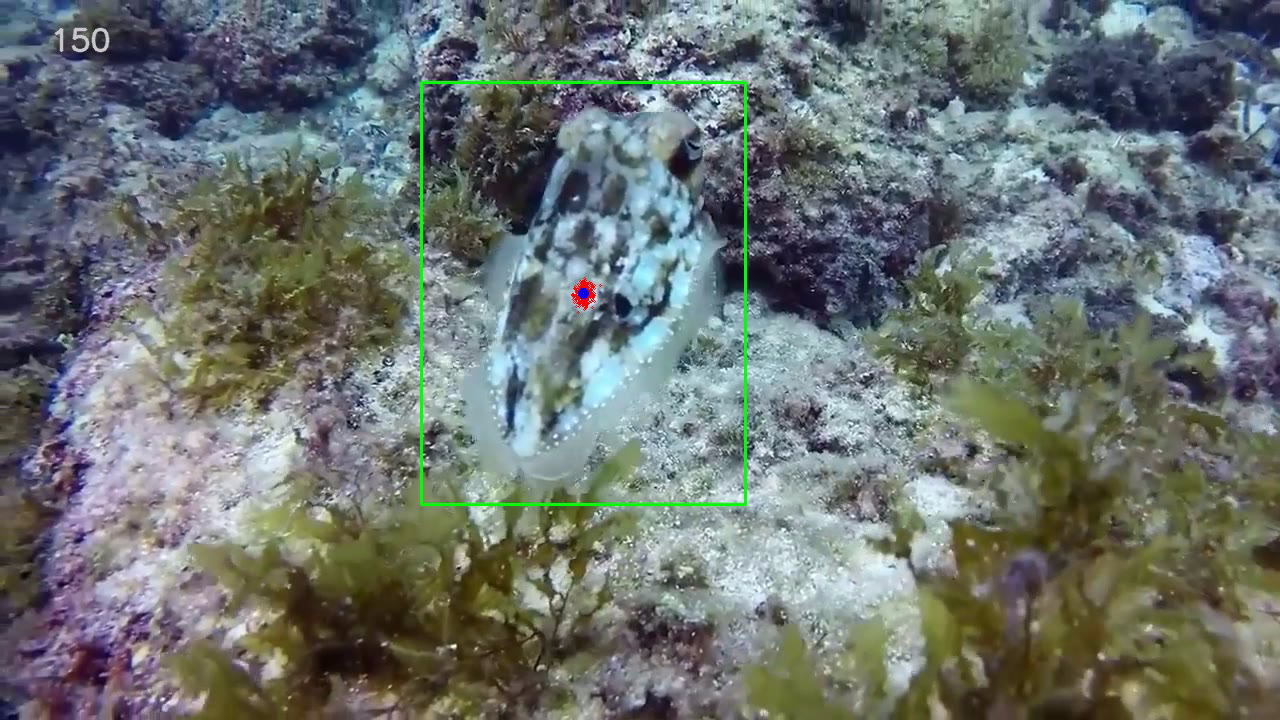
\includegraphics[scale=0.15]{result_pf_valid_4.png}}}
	\\
	\subfloat[Frame 200]{{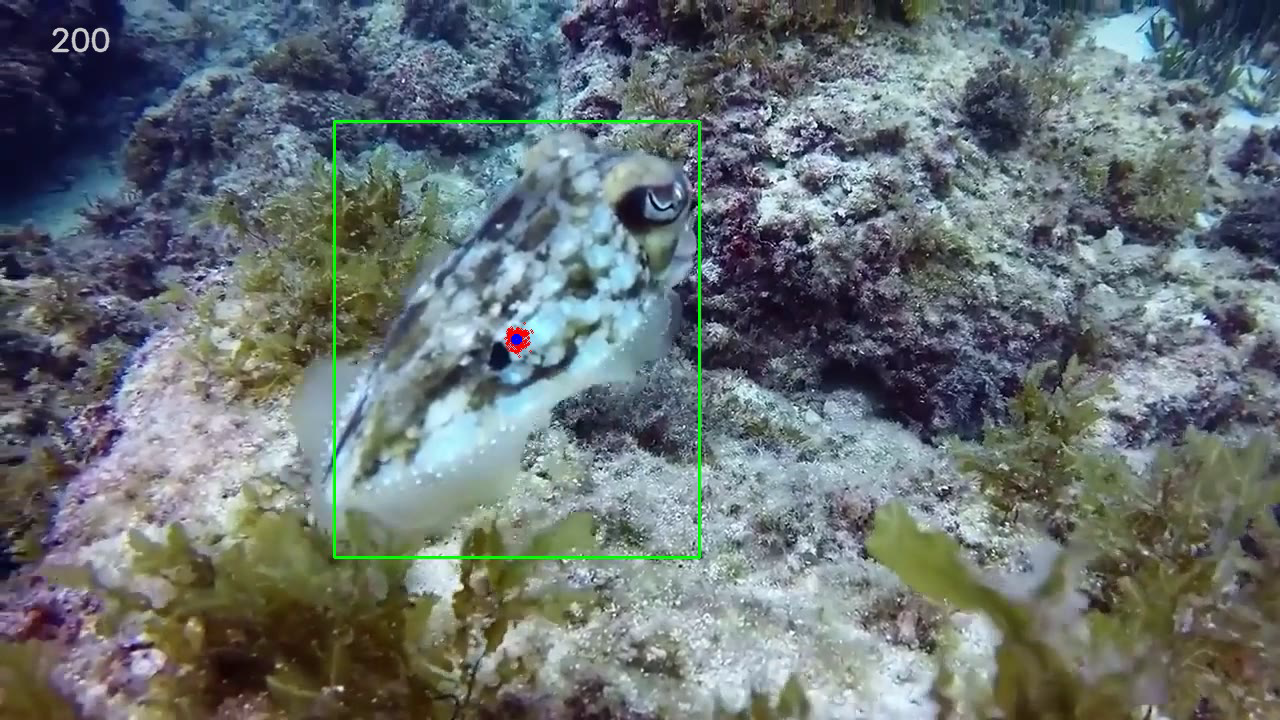
\includegraphics[scale=0.15]{result_pf_valid_5.png}}}
	\hspace{0.1cm}
	\subfloat[Frame 250]{{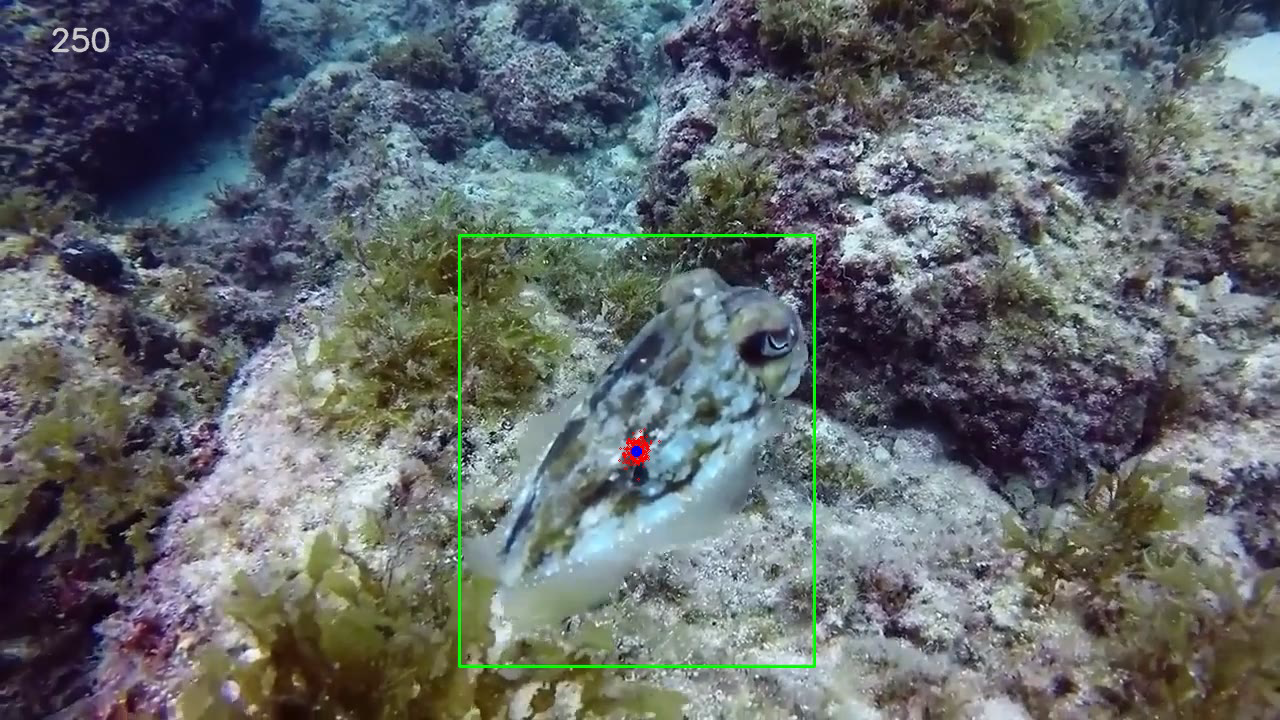
\includegraphics[scale=0.15]{result_pf_valid_6.png}}}
\caption{Exemple de résultats obtenus par notre filtre à particule.}
\label{fig:pf_results}
\end{figure}
\FloatBarrier

\begin{figure}[!htbp]
\center
	\subfloat[Frame 25]{{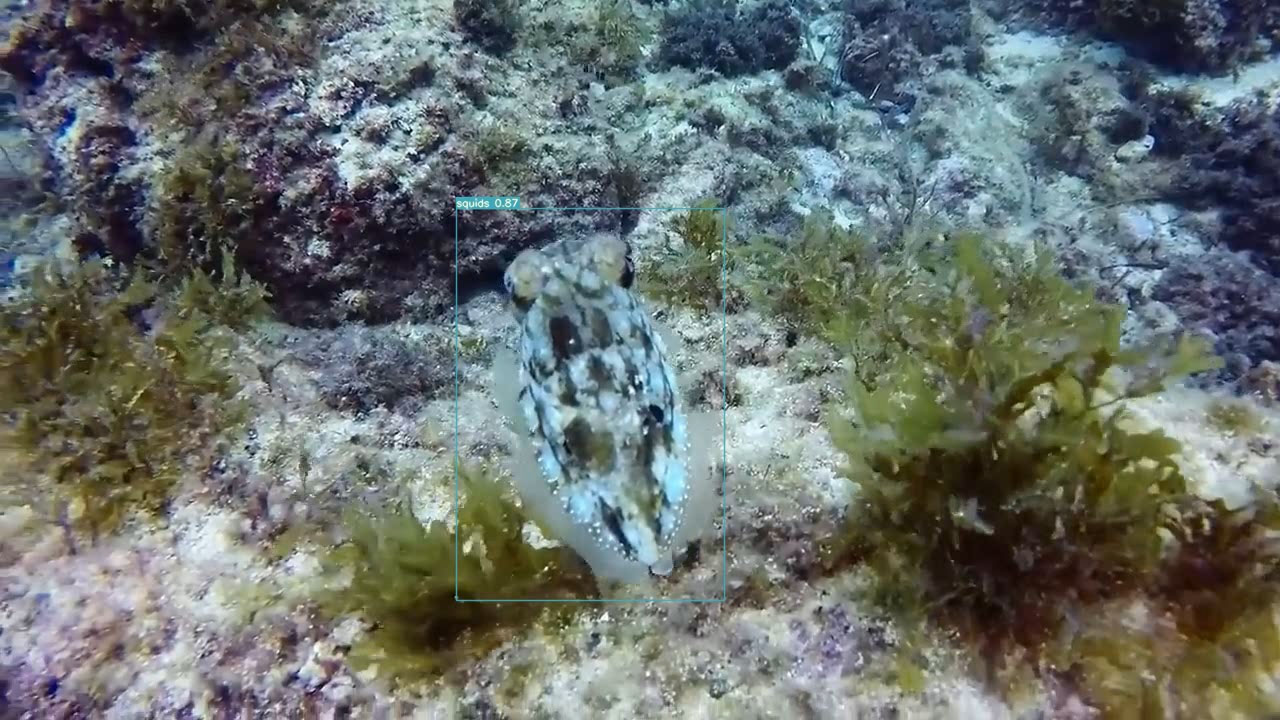
\includegraphics[scale=0.15]{result_yolo_valid_1.jpg}}}
	\hspace{0.1cm}
	\subfloat[Frame 50]{{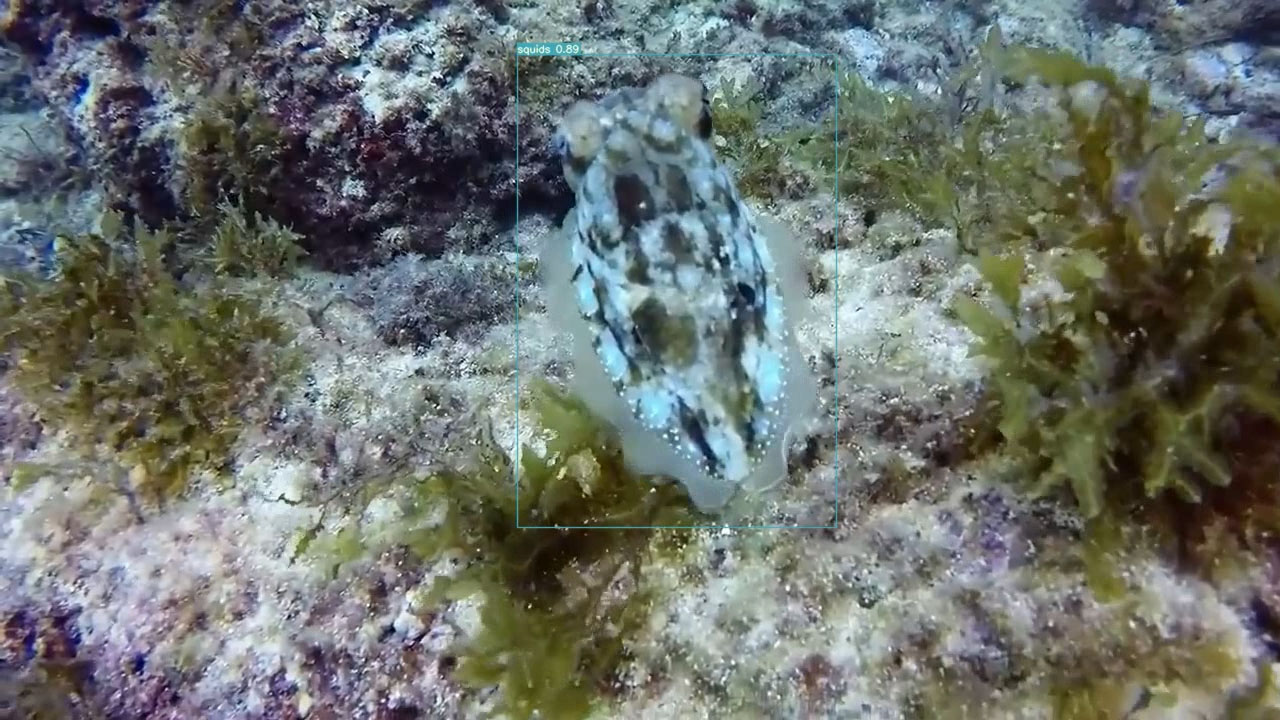
\includegraphics[scale=0.15]{result_yolo_valid_2.jpg}}}
	\\
	\subfloat[Frame 100]{{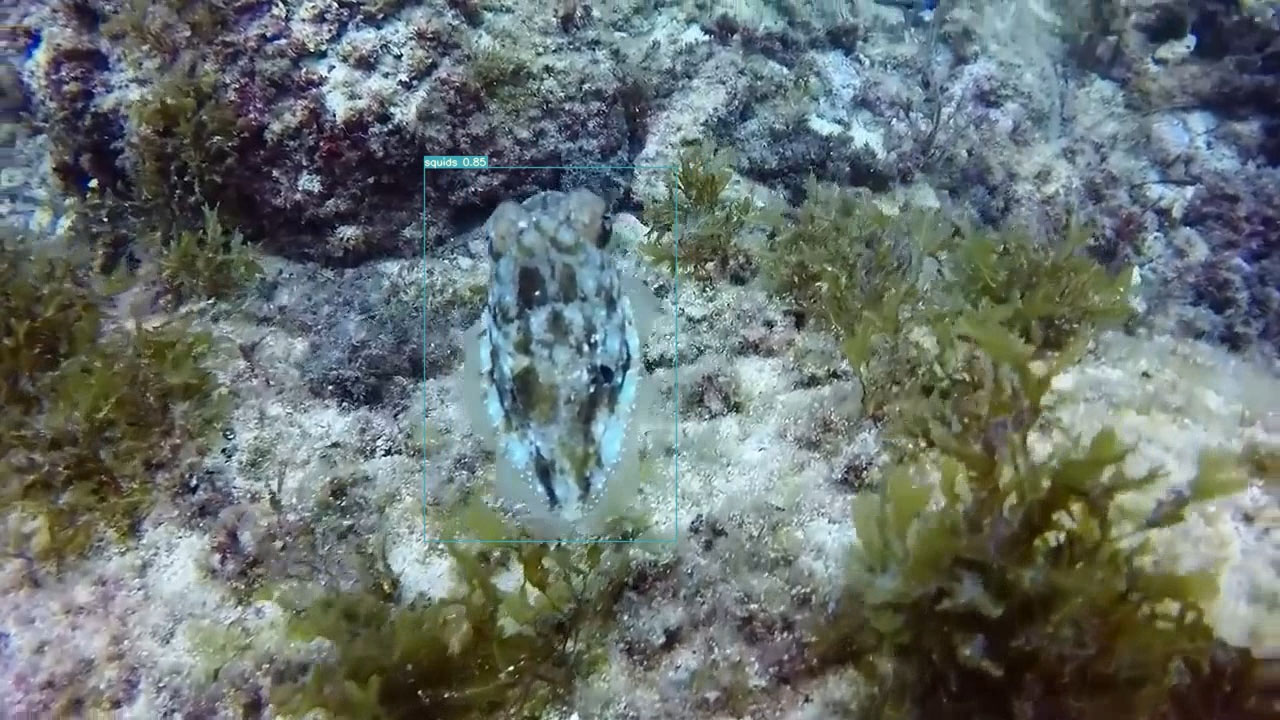
\includegraphics[scale=0.15]{result_yolo_valid_3.jpg}}}
	\hspace{0.1cm}
	\subfloat[Frame 150]{{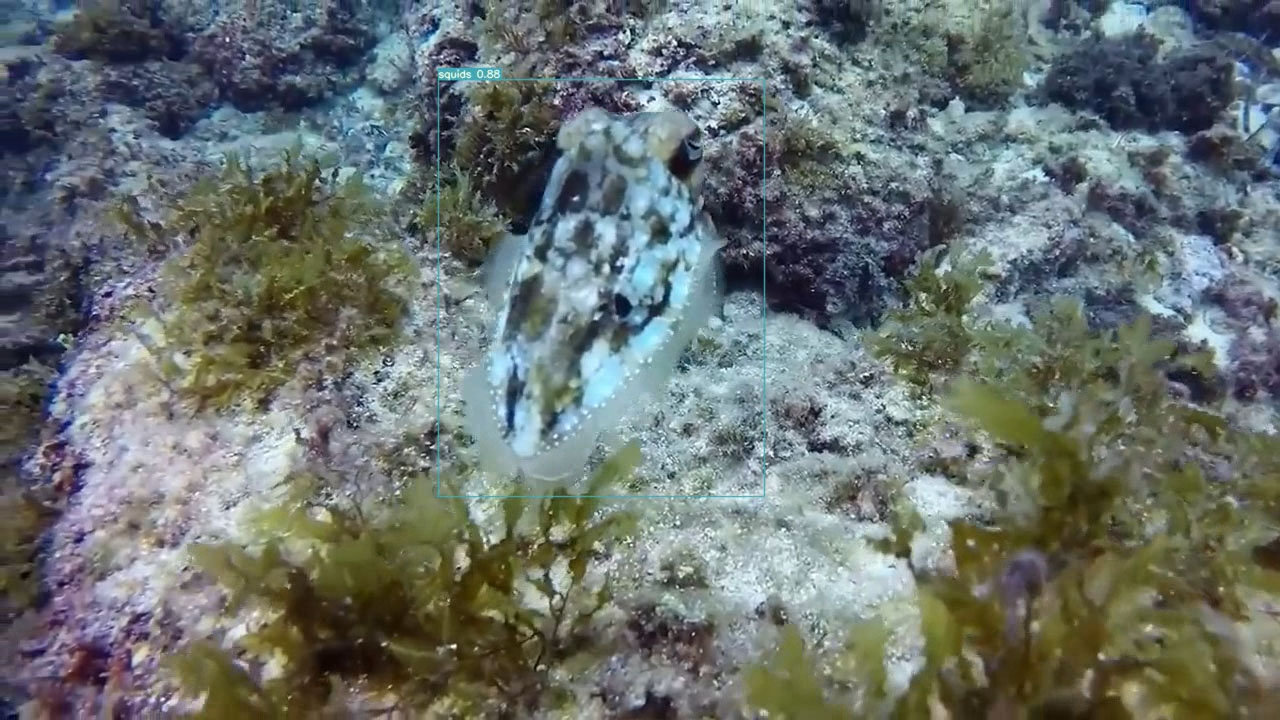
\includegraphics[scale=0.15]{result_yolo_valid_4.jpg}}}
	\\
	\subfloat[Frame 200]{{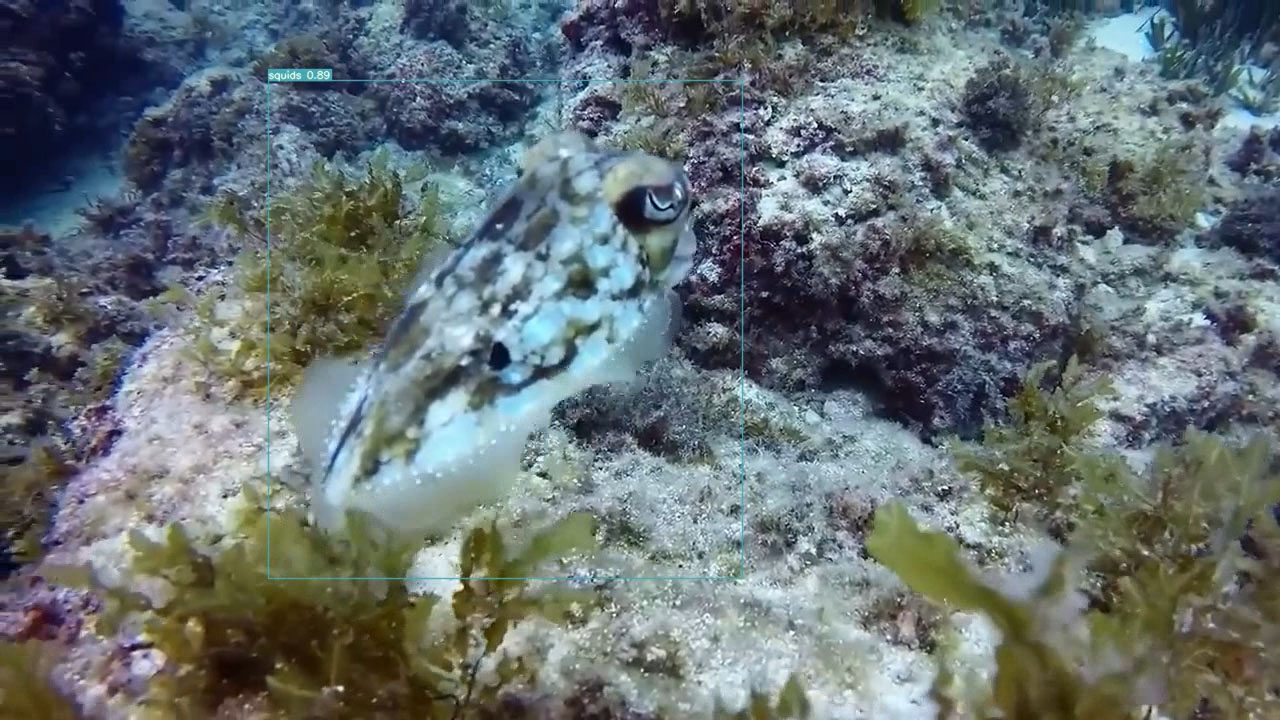
\includegraphics[scale=0.15]{result_yolo_valid_5.jpg}}}
	\hspace{0.1cm}
	\subfloat[Frame 250]{{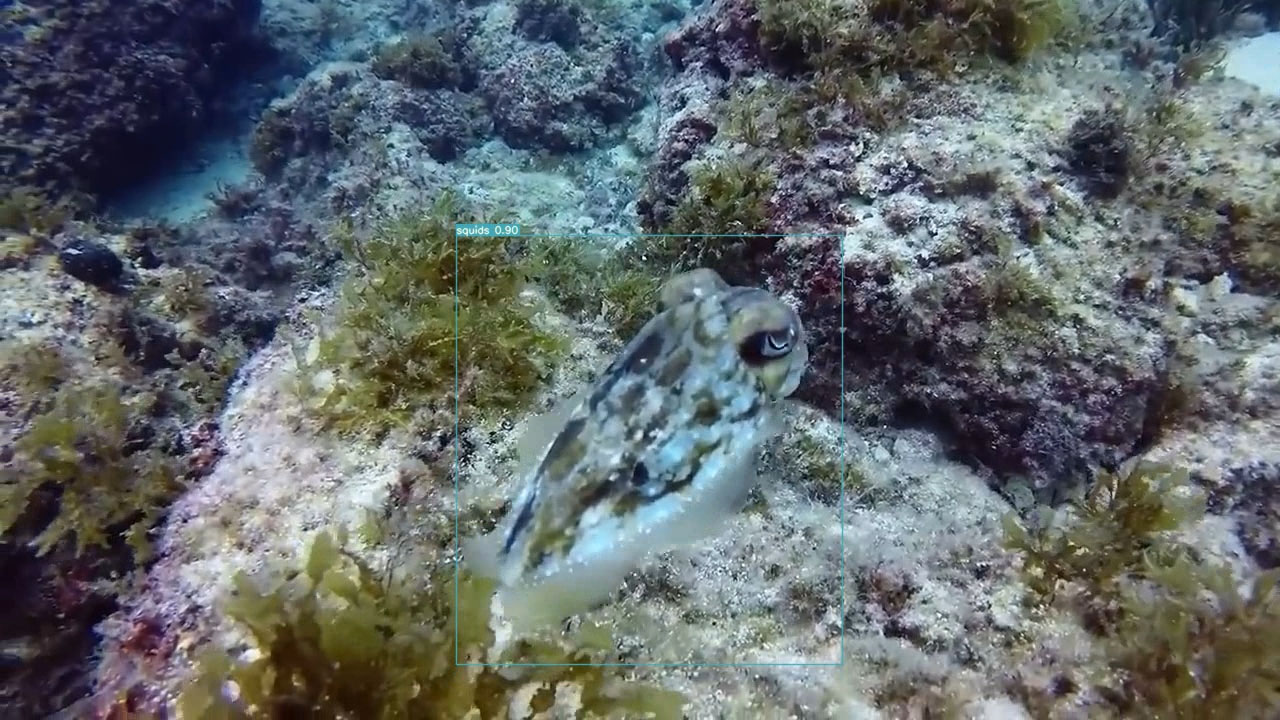
\includegraphics[scale=0.15]{result_yolo_valid_6.jpg}}}
\caption{Exemple de résultats obtenus par YOLOv7.}
\label{fig:yolo_results}
\end{figure}
\FloatBarrier


Les courbes de déplacement de la seiche dans les figure \ref{fig:trajX_pf}, \ref{fig:trajY_pf}, \ref{fig:trajX_yolo} et \ref{fig:trajY_yolo} illustrent un exemple de détection continue dans une séquence.\\
Dans la figure \ref{fig:trajX_pf}, nous comparons la trajectoire de la seiche suivi par le filtre à particule (couleur violette) aux positions définies manuellement (couleur or) dans la direction des x, tandis que dans la figure \ref{fig:trajY_pf} nous comparons les deux trajectoires dans la direction des y.\\
De même, dans la figure \ref{fig:trajX_yolo} nous comparons la trajectoire de la seiche suivi par YOLOv7 (couleur bleu) aux positions définies manuellement (couleur or) dans la direction des x, tandis que dans la figure \ref{fig:trajY_yolo} nous comparons les deux trajectoires dans la direction des y.\\
\\
La distance entre la trajectoire automatique et manuelle indique la précision de l'algorithme, ce qui donne pour la séquence une erreur moyenne globale de 21 pixels pour le filtre à particule, calculé sur les 288 frames de la séquence où la seiche a été détectée, et 12 pixels pour YOLOv7, calculé sur les 292 frames de la séquence où la seiche a été détectée.\\
La méthode de détection avec filtre à particule semble détecter la seiche dans 98\% de la séquence, et la méthode de détection avec YOLOv7 dans 100\% de la séquence.

\begin{figure}[!htbp]
\center
	\subfloat{{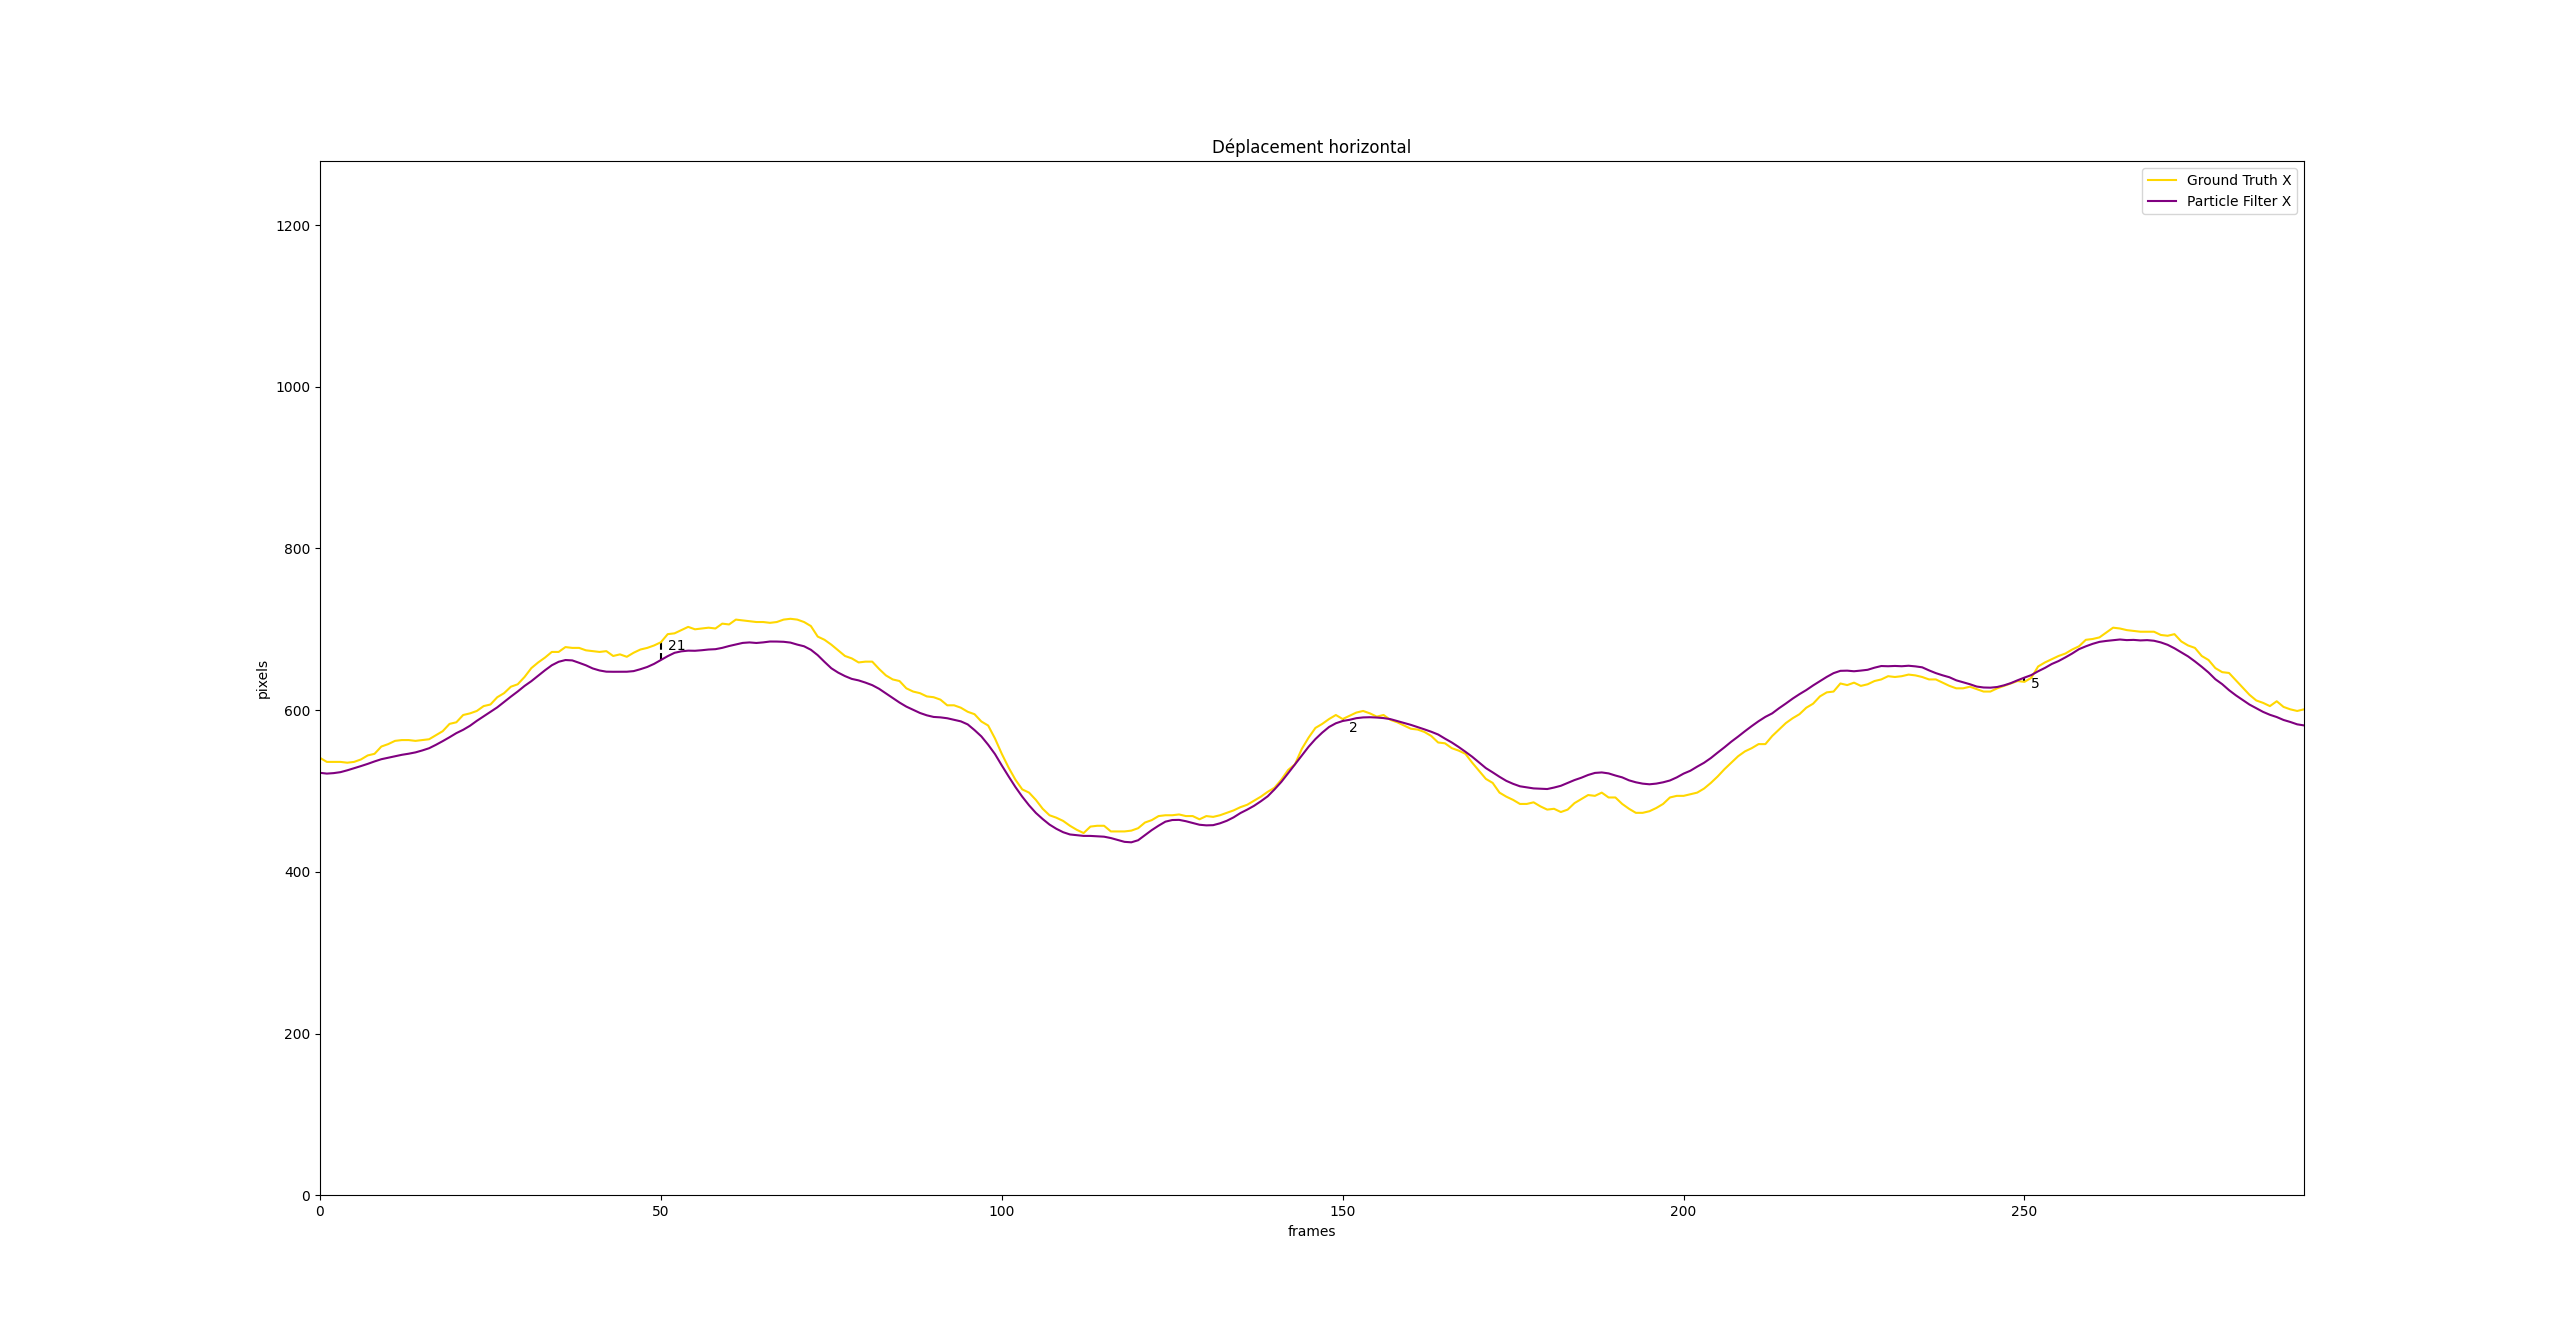
\includegraphics[scale=0.3]{X_displacement_pf.png}}}
\caption{Trajectoire avec le filtre à particule sur les X}
\label{fig:trajX_pf}
\end{figure}
\FloatBarrier

\begin{figure}[!htbp]
\center
	\subfloat{{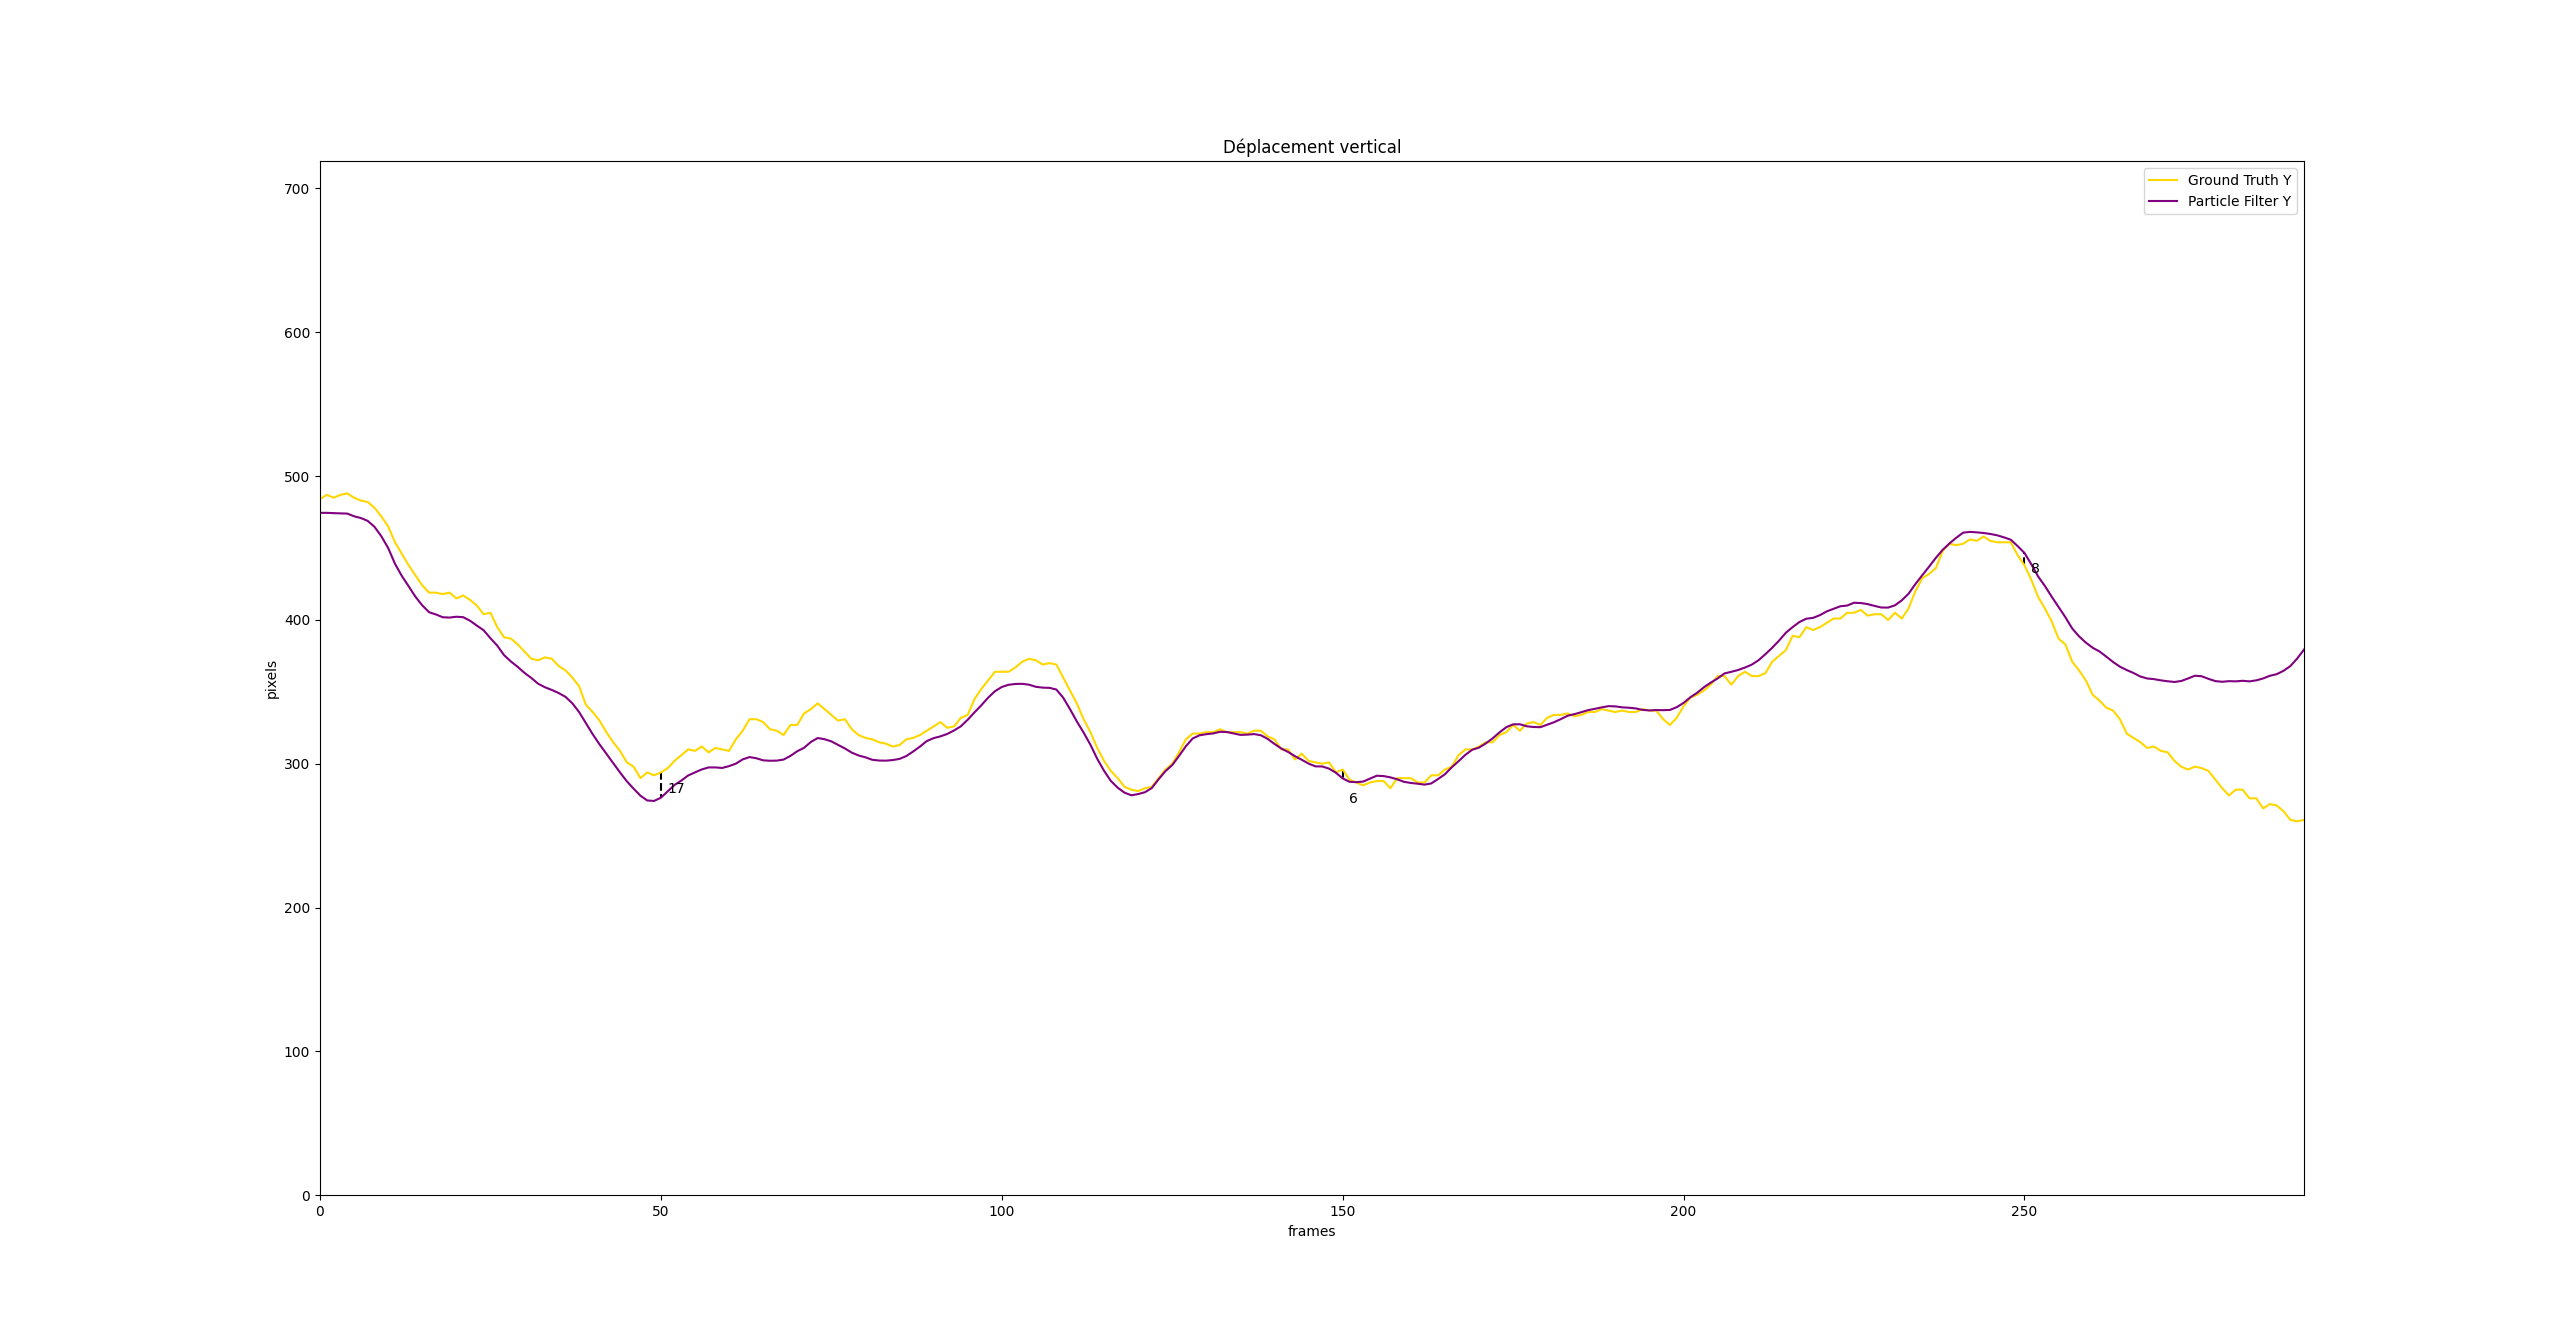
\includegraphics[scale=0.3]{Y_displacement_pf.png}}}
\caption{Trajectoire avec le filtre à particule sur les Y}
\label{fig:trajY_pf}
\end{figure}
\FloatBarrier

\begin{figure}[!htbp]
\center
	\subfloat{{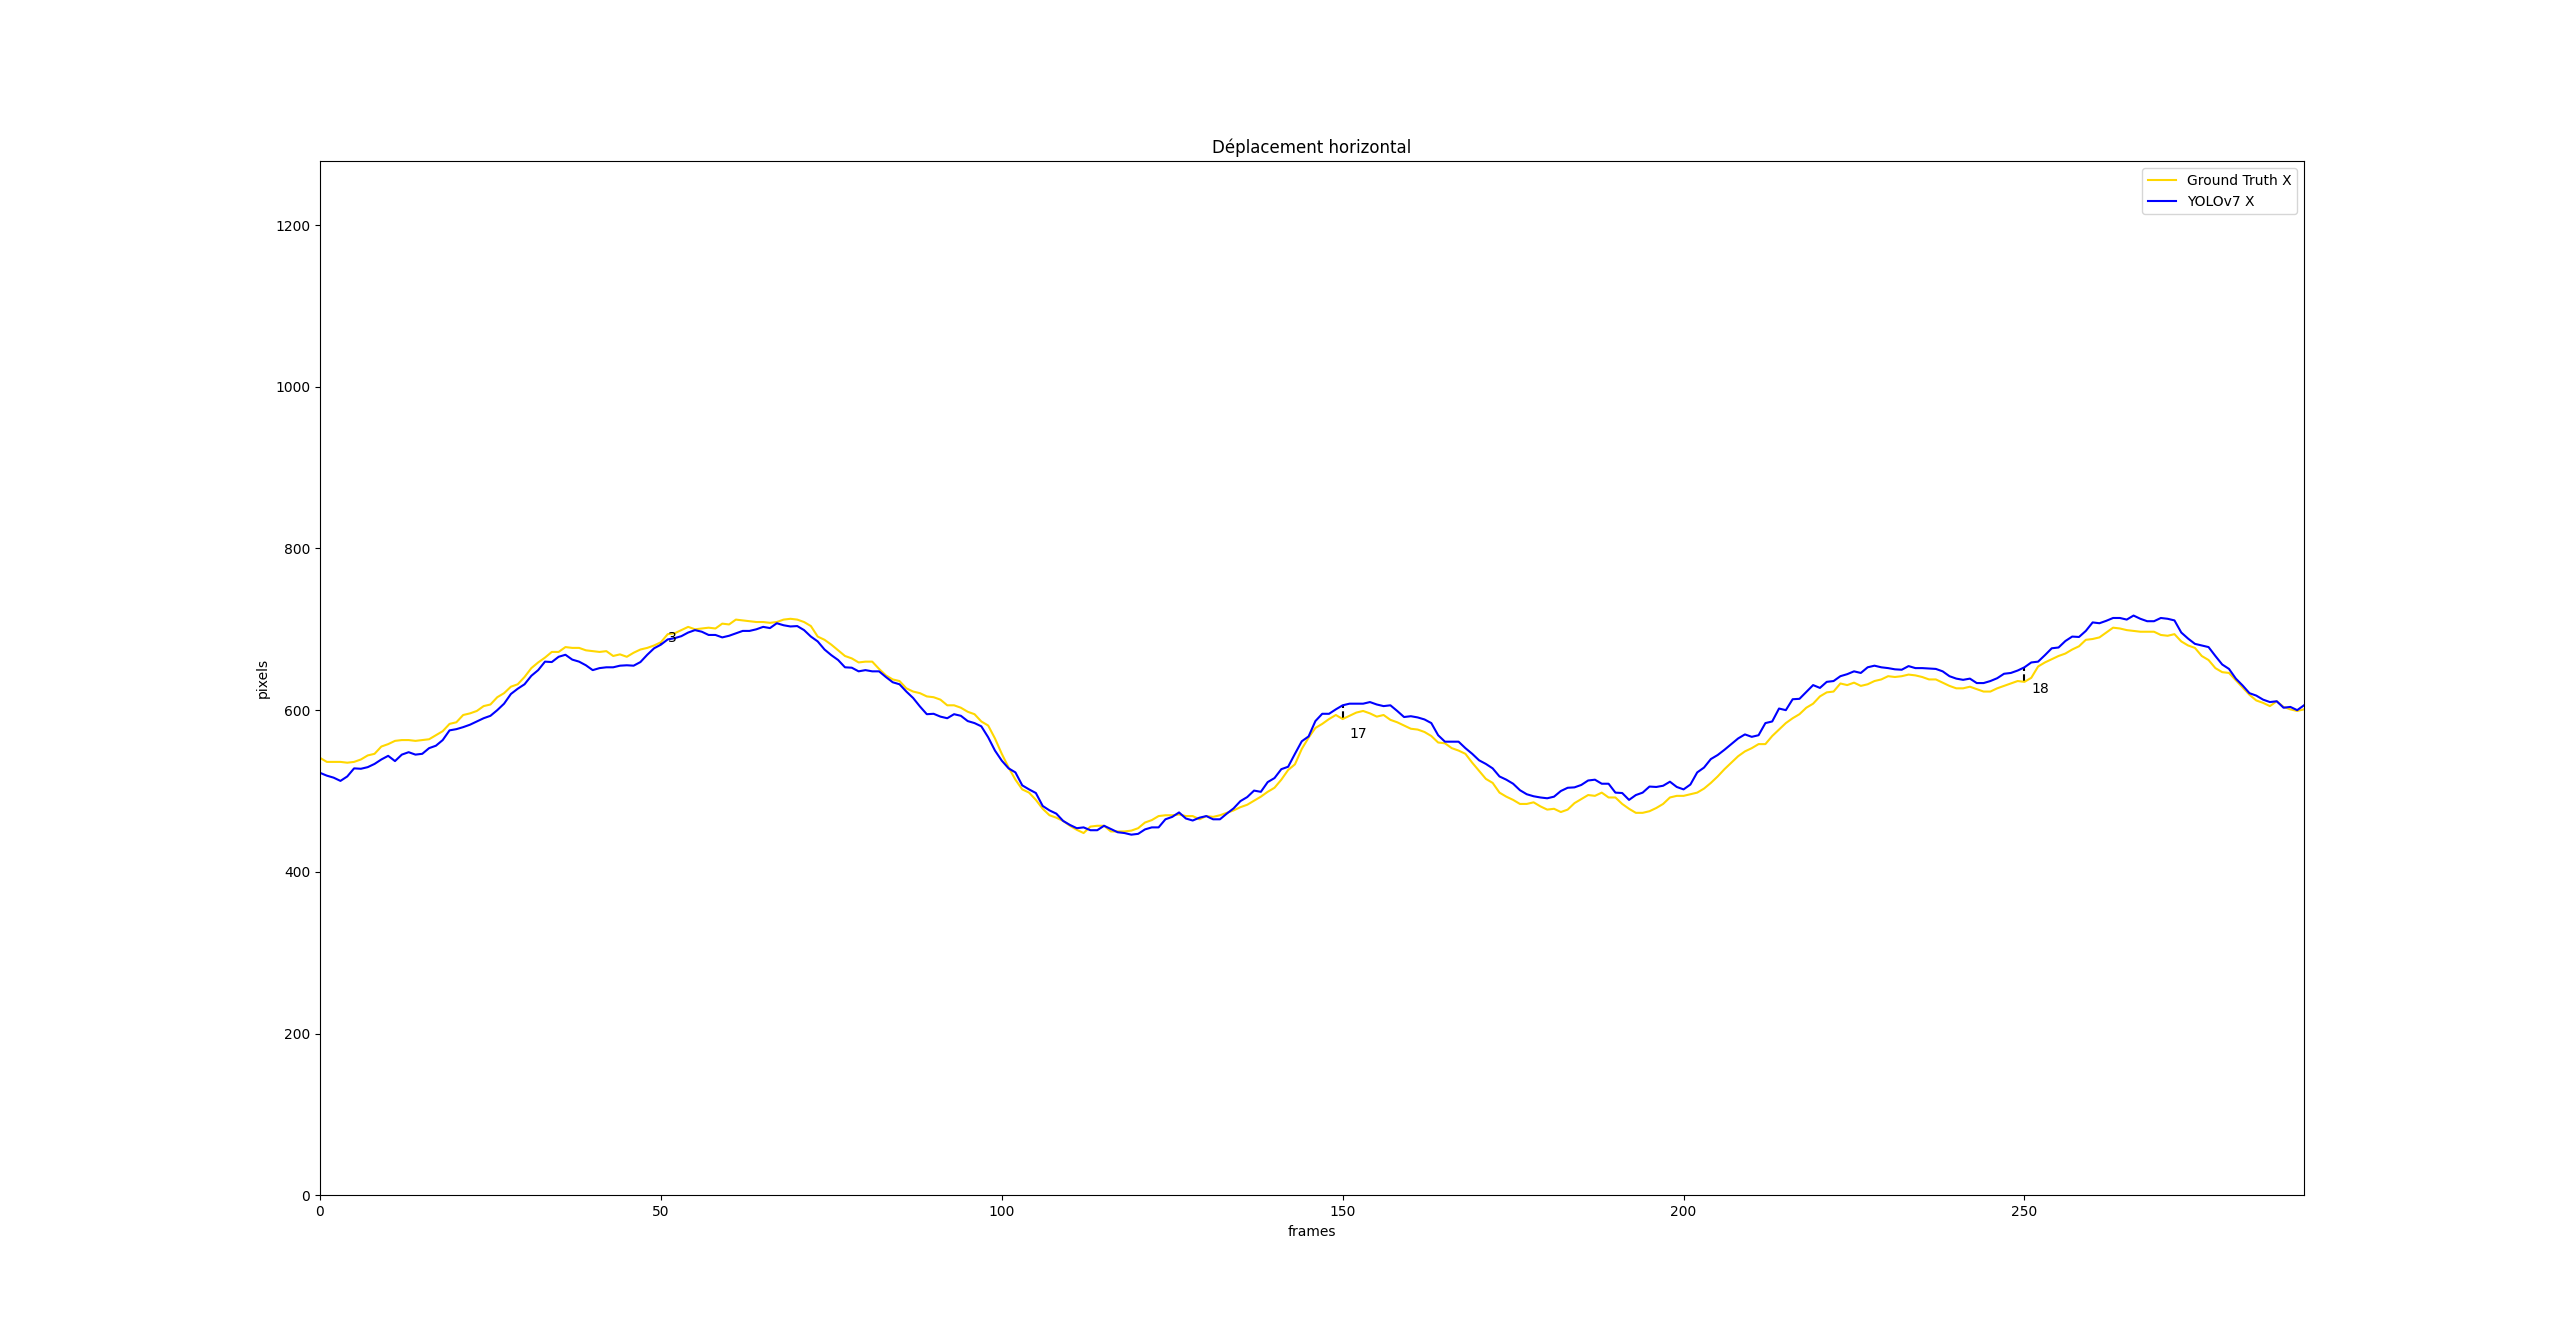
\includegraphics[scale=0.3]{X_displacement_yolo.png}}}
\caption{Trajectoire avec YOLOv7 sur les X}
\label{fig:trajX_yolo}
\end{figure}
\FloatBarrier

\begin{figure}[!htbp]
\center
	\subfloat{{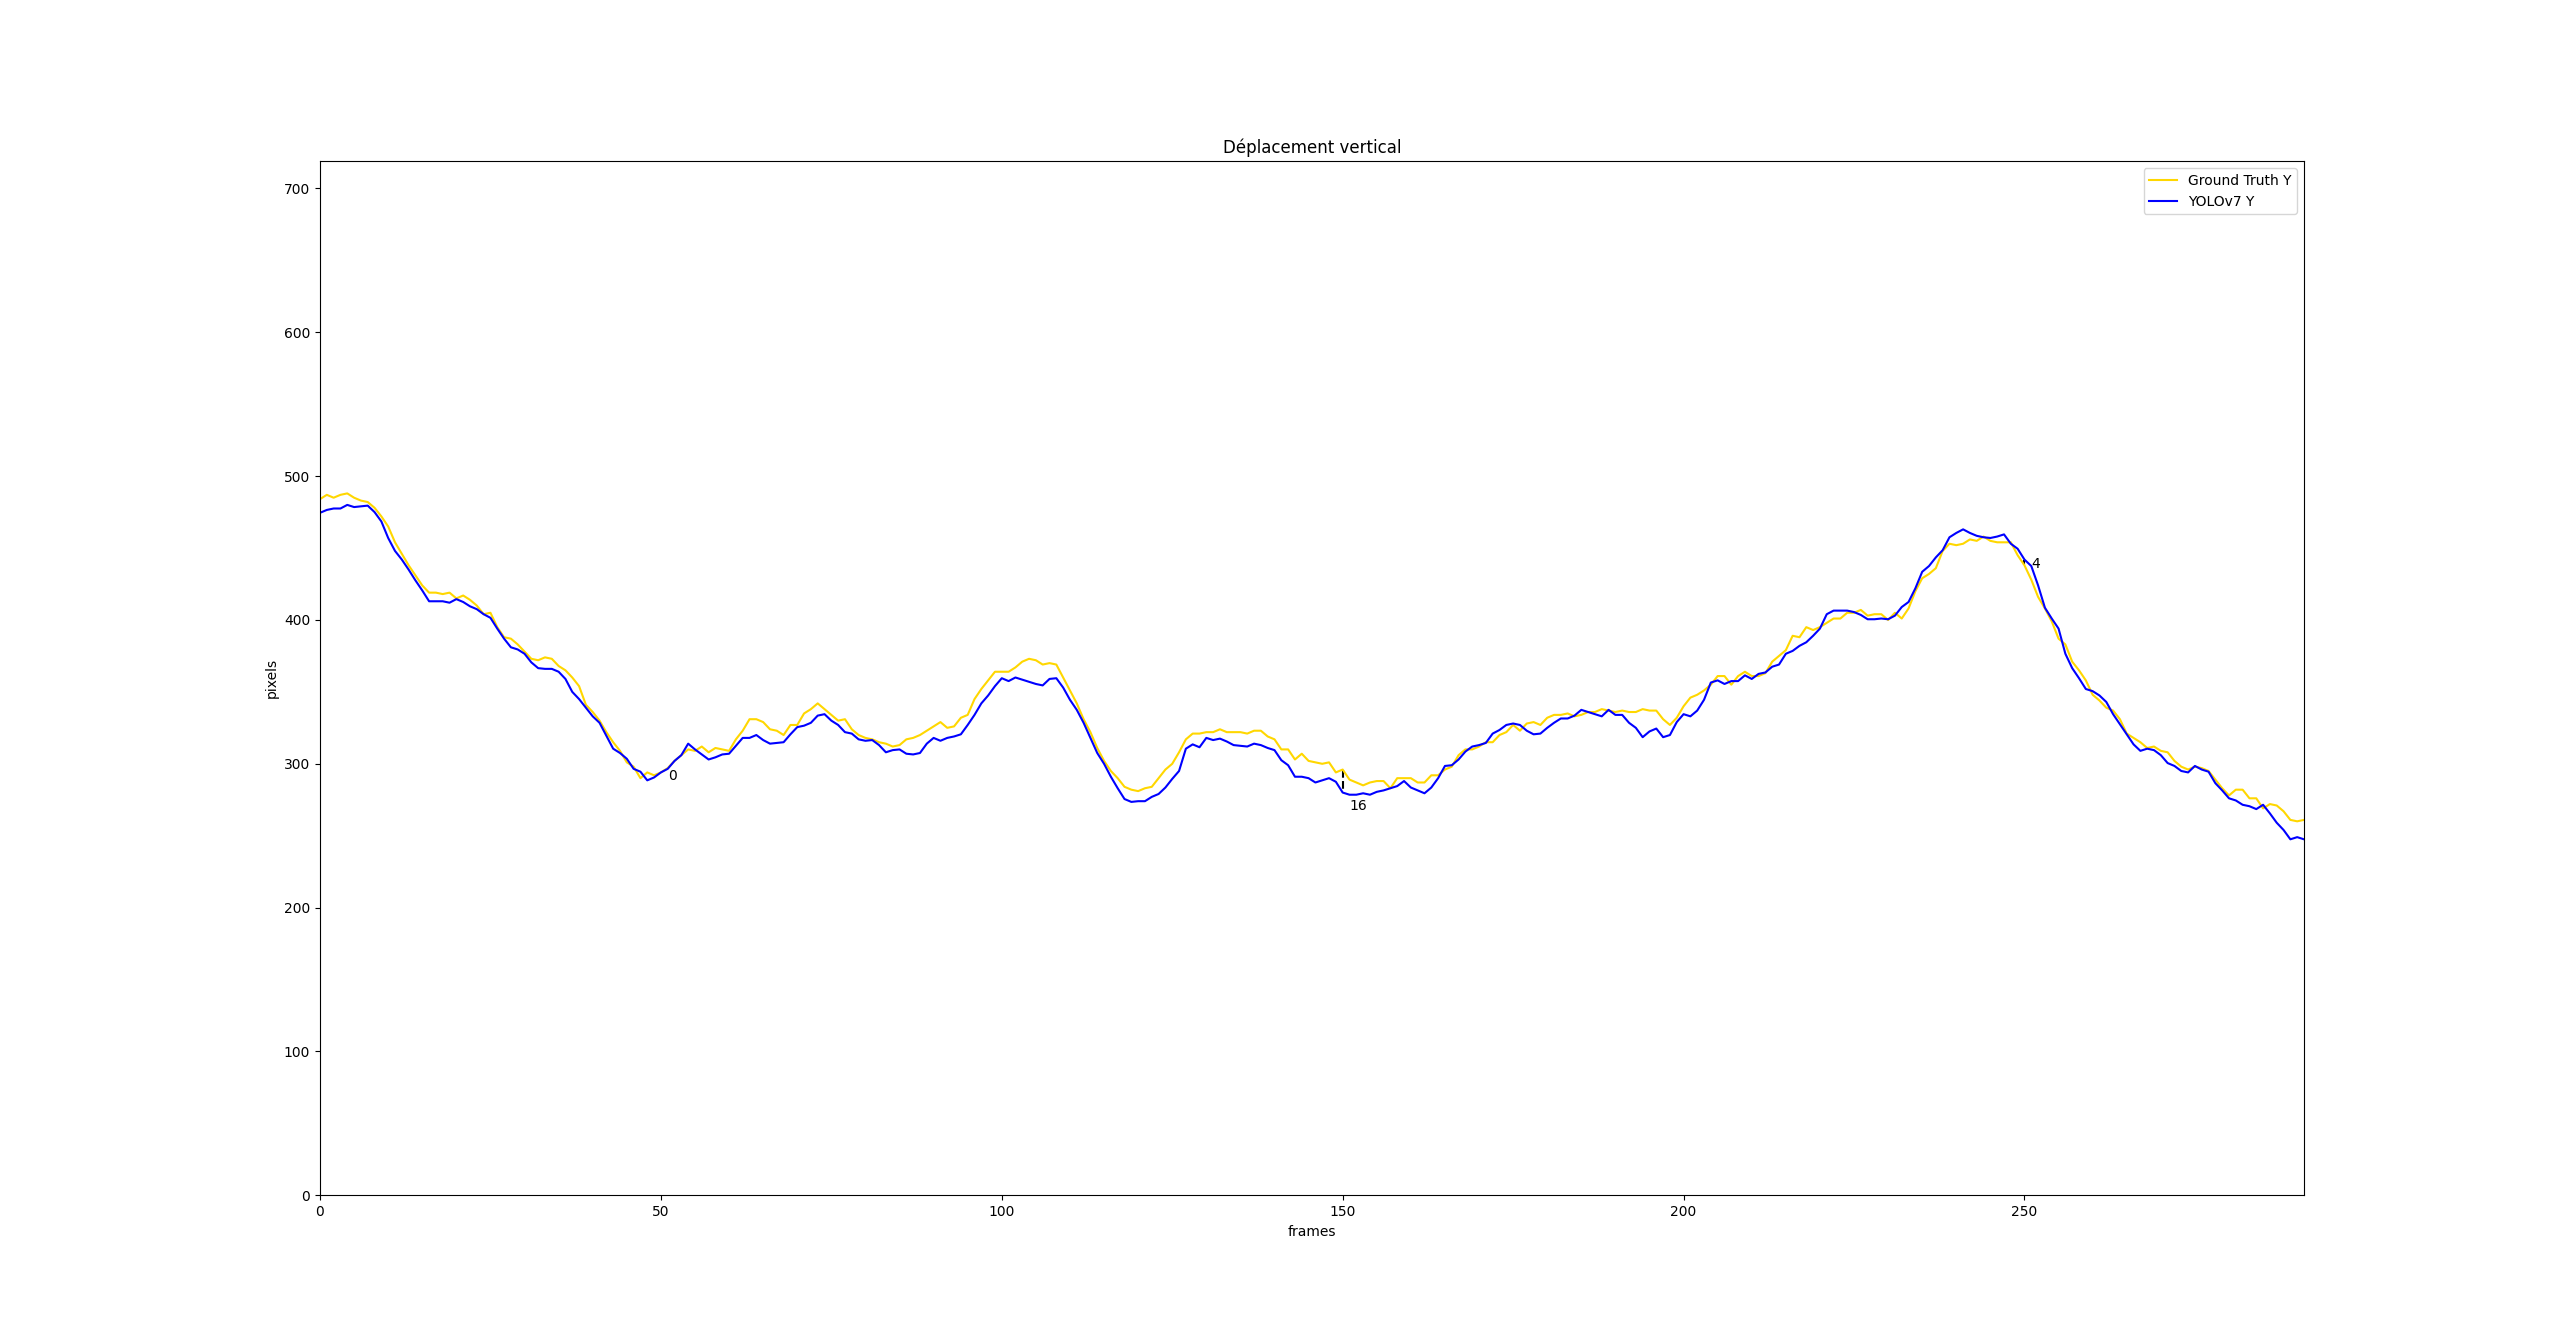
\includegraphics[scale=0.3]{Y_displacement_yolo.png}}}
\caption{Trajectoire avec YOLOv7 sur les Y}
\label{fig:trajY_yolo}
\end{figure}
\FloatBarrier
 

Cependant, la détection avec le filtre à particule peut diverger, comme illustré dans la figure \ref{fig:pf_diverg_results}. Cette divergence peut s'expliquer de plusieurs manières. Elle peut provenir d'une accumulation d'erreur lors du suivi, ou bien d'une paramétrisation du logiciel non optimale, ou encore de la seiche qui n'est que sur une petite portion de la bounding box, ce qui a pour effet de beaucoup plus représenter l'arrière plan et donc mettre un poids plus élevé sur ce qui ressemble à l'arrière plan lors de l'étape de calcul des poids.

\begin{figure}[!htbp]
\center
	\subfloat{{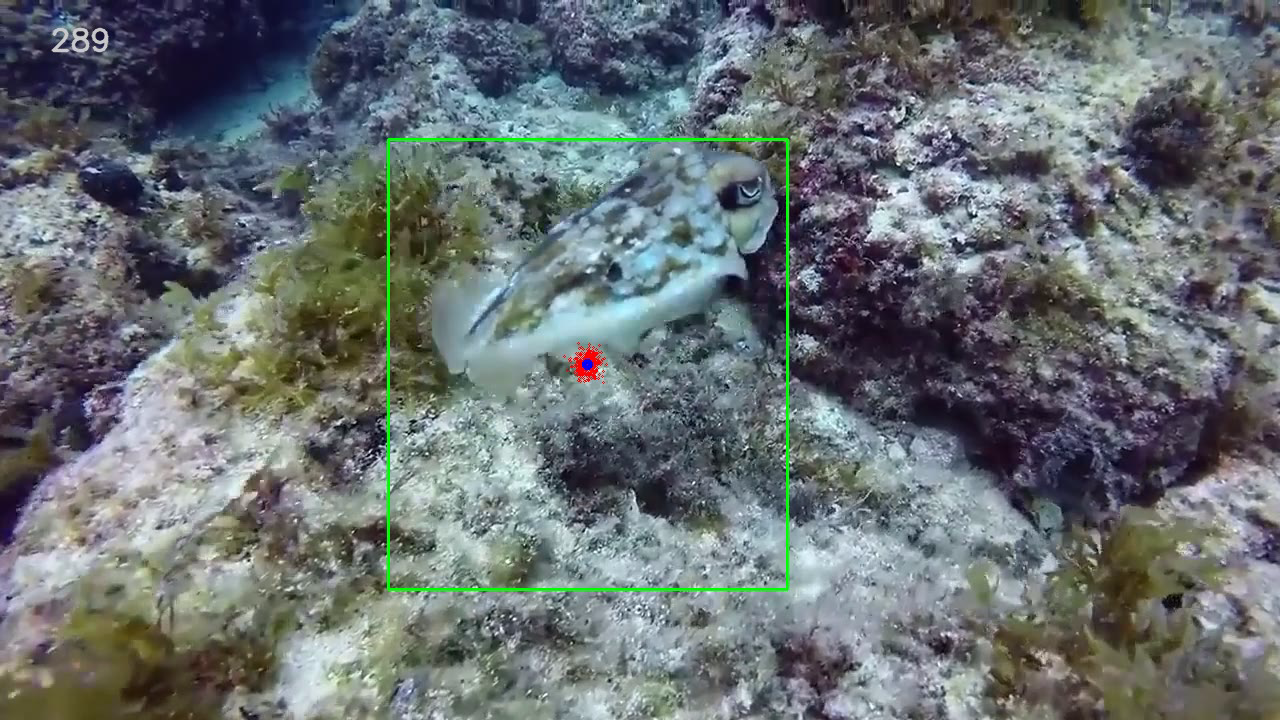
\includegraphics[scale=0.15]{result_pf_invalid_1.png}}}
	\hspace{0.1cm}
	\subfloat{{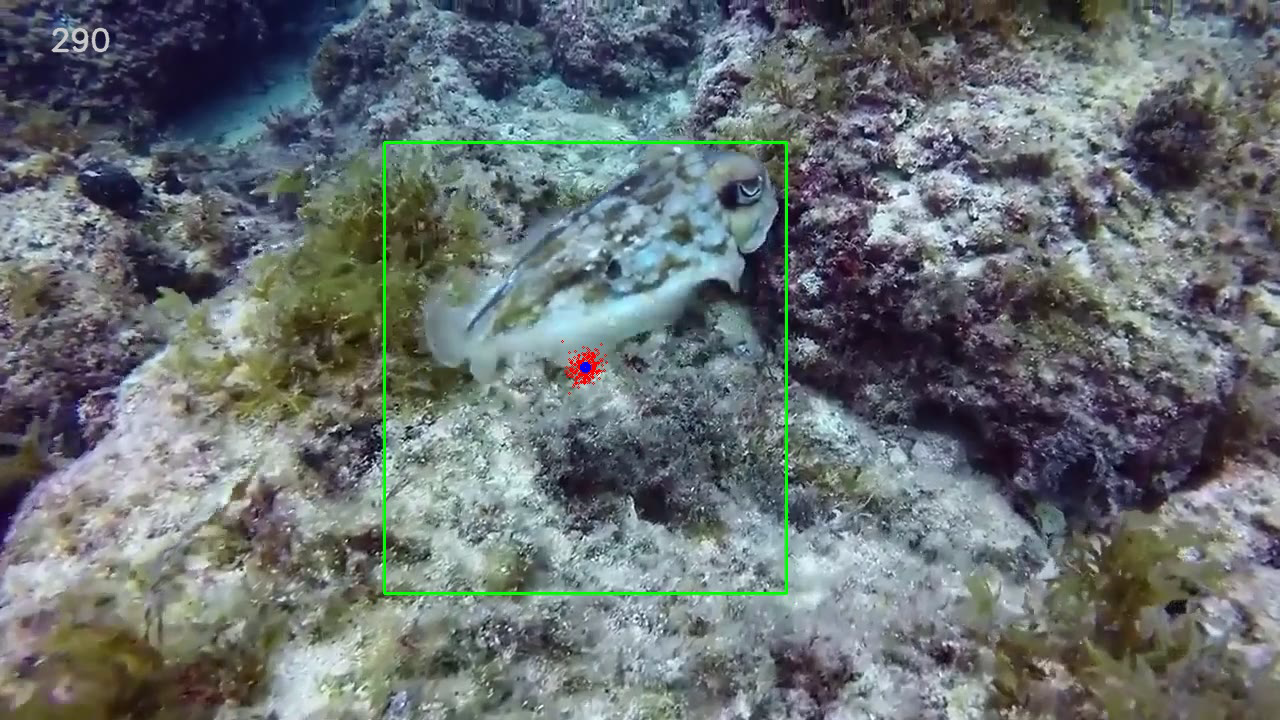
\includegraphics[scale=0.15]{result_pf_invalid_2.png}}}
	\\
	\subfloat{{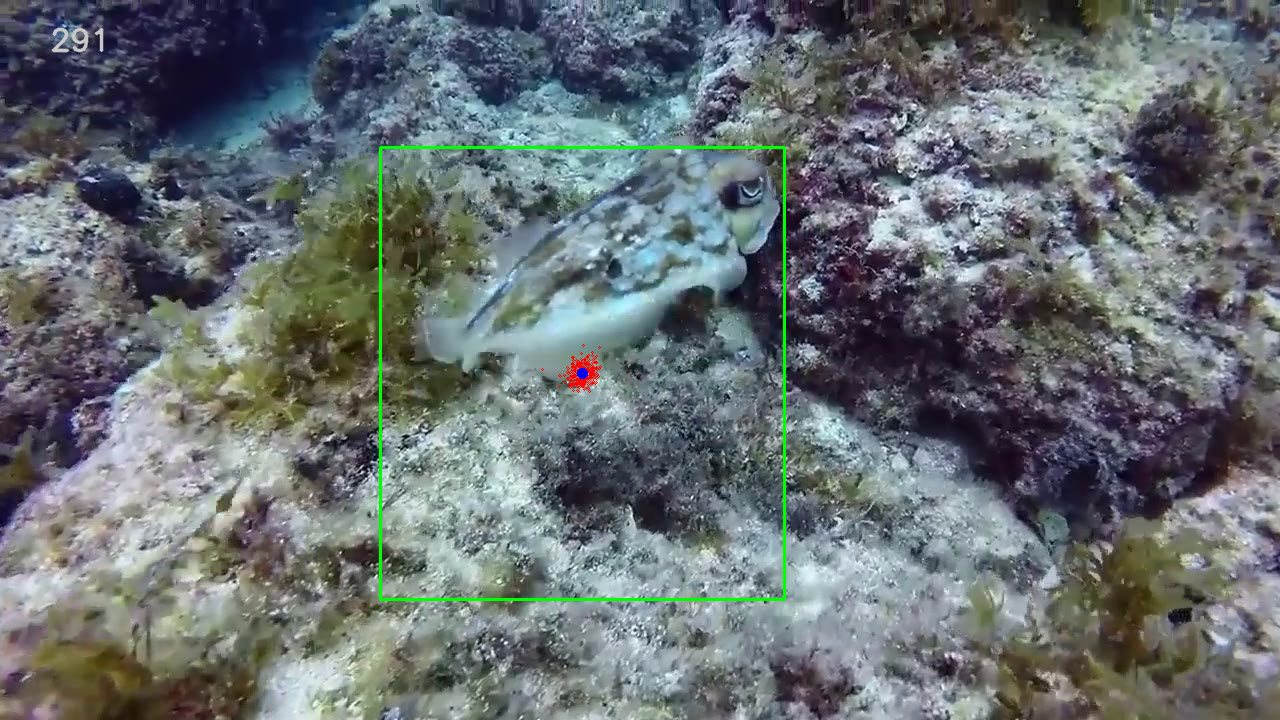
\includegraphics[scale=0.15]{result_pf_invalid_3.png}}}
	\hspace{0.1cm}
	\subfloat{{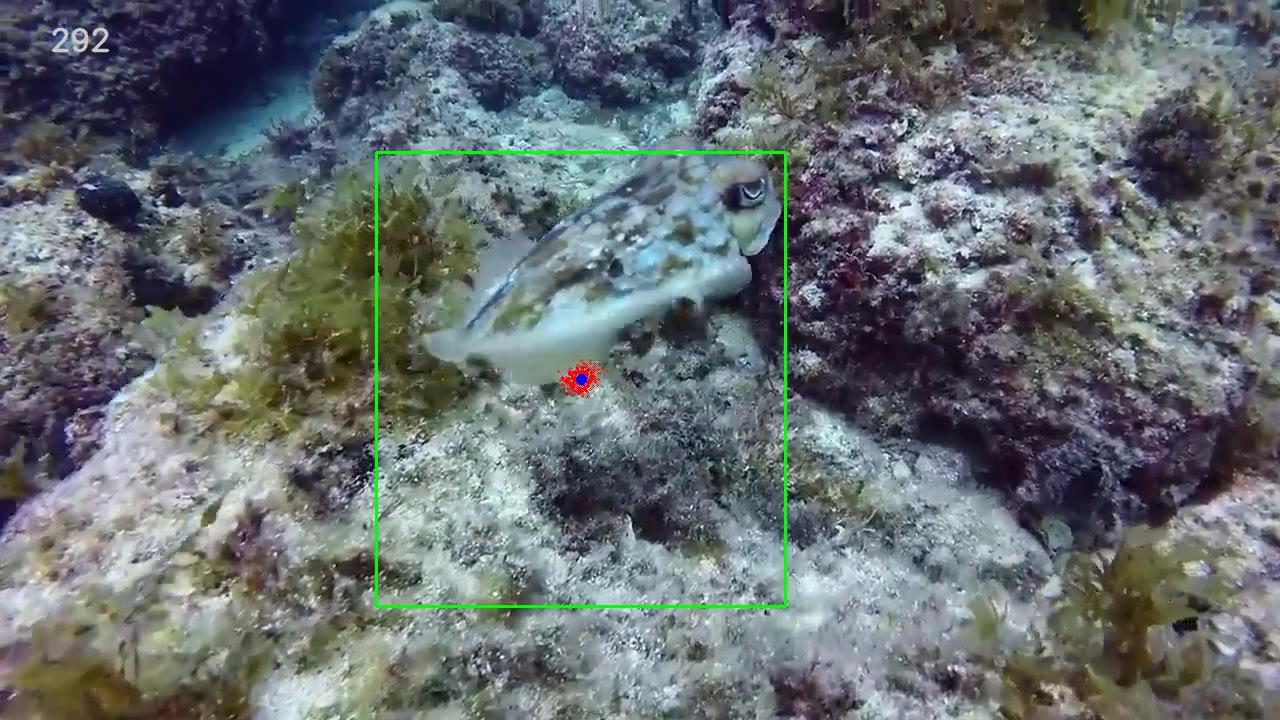
\includegraphics[scale=0.15]{result_pf_invalid_4.png}}}
\caption{Exemple de résultats divergeant obtenus par notre filtre à particule.}
\label{fig:pf_diverg_results}
\end{figure}
\FloatBarrier

\clearpage